
\chapter{ \uppercase {Residual Monte Carlo Treatment of the Time Variable}}
\label{sec:time}
Another area of potential improvement for the HOLO method is in the time discretization
of the system.  We have investiaged using MC integration of the time derivative in the HO
solver and introducing extra consistency terms into the LO equations.  The goal is to produce a more accurate solution in optically
thin regions where particles transport a long distance.  A potential application is in 
stellar atmosphere calculations.  In optically thin regions, the MC
integration of the time-variable by IMC can produce greater accuracy, whereas an implicit
Euler discretization will result in artificially fast propagation of energy.  We hope to improve
the efficiency of MC calculations in thin regions with the ECMC method while still preserving the
accuracy of a MC treatment in the time variable.  The time variable is included in
the trial space for ECMC and the LO equations are closed consistently.  We
will not be performing adaptive refinement in time, so maintaining exponential convergence
may not be possible.  However, we still expect the residual MC formulation of the ECMC method
to show improvement over standard MC.

\section{Modifications to the HO equations}
\label{sec:time_ho}

Inclusion of the time variable $t$ in the trial space used by ECMC allows for no discretization of the
transport operator $\B L$.  The transport operator, applied to the continuos intensity $I$
becomes,
\begin{equation}
   \B LI(x,\mu,t) = \frac{1}{c}\pderiv{I}{t} + \sigma_t I + \mu \pderiv{I}{x}
\end{equation}
The emission source is still treated with an implicit Euler discretization, which is
simlar to the approximation used in IMC. 

The ECMC algorithm is still specified the same as in Sec.~\ref{sec:???}, however the residual
source and MC tracking are now modified.   Each batch is still estimating the error in the
estimate, but now the time variable must be included in the inversion of the $\B L$
operator.  The process of sampling and tracking in time
step is detailed in literature\cite{wollaber_review,fnc,wollaber_thesis,cj_thesis}, but a
brief outline is given in the following sections. 

\subsection{The Doubly-Discontinuous Trial Space}

It is necessary to define the time trial space so that we can explicitly define the
residual for sampling.  This trial space is similar to the LDD trial space used for the space variable
in Sec.~\ref{sec:lo_closure_LDDTRIAL???}, however the solution is a constant value over
the interior of the time step. This step, doubly-discontinuous trial space is defined as
\begin{equation}\label{eq:time_space}
    \tilde I(x,\mu,t) = \left \{ \begin{matrix} 
        \tilde I^{n}(x,\mu)  & t = t^n \\ 
        \overline I(x,\mu)  & t \in (t^{n},t^{n+1}) \\               
        & t = t^{n+1}
             \end{matrix}           \right.
\end{equation}
where we have used $\overline I$ to denote the time-averaged value of the intensity over
the interior of the time step and $\tilde I(x,\mu)$ is an LDFE projection in $x$ and
$\mu$.  An illustration of the time variable for this trial space
is depicted in Fig.~\ref{fig:dd_time}.    There is a projection error in that we have used the LDFE space-angle
projection to represent the intensity from the previous time step.  However, with
sufficient noise reduction and mesh resolution this should not be a large error as
compared to IMC.
\begin{figure}[H]
    \centering
    \begin{center}
        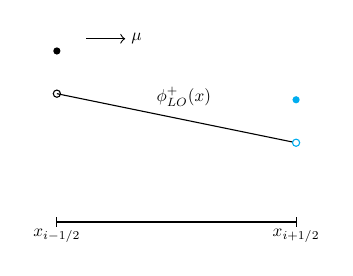
\begin{tikzpicture}[scale=0.62, every node/.style={transform shape}]
            \draw (1.0,4.0) node[fill,circle,inner sep=0pt,minimum
            size=4.2pt] {};
            \draw [->] (1.6,4.25) -- (2.4,4.25) node[anchor=west] {$\mu$};
            \draw (1.0,0.4) -- (1.0,0.6) node[below, pos=0.4] {$x_{i-1/2}$};
            \draw (5.90,0.4) -- (5.90,0.6) node[below, pos=0.4] {$x_{i+1/2}$};
            \node at (3.6,3.06) {$\phi_{LO}^+(x)$};
            \draw [thick] (1.0,0.5) -- (5.9,0.5) node[anchor=north west] {};
            \filldraw[color=black, fill=white] (1,3.1250) circle (2.1pt);
            \draw (1.0,3.125) -- (5.90,2.120);
            \filldraw[color=cyan, fill=white] (5.9,2.120) circle (2.1pt);
            \draw (5.9,3.0) node[cyan,fill,circle,inner sep=0pt,minimum size=4.2pt] {};
        \end{tikzpicture}
    \end{center}
    \caption{Step doubly-discontinuous representation of $t$ for the HO solution.}
    \label{fig:dd_time}
\end{figure}

The choice of this trial space will provide a projection for all the desired unknowns to exactly produce the moment
equations, i.e., the time-averaged, end of time step, and previous time step values for
the intensity.  Temporally, these are the only unknowns that appear in equations that have
been integrated over a time step to produce a balance statement.  Another reason for this
choice is that it allows for infrastructure for computing the residual from the
time-discrete case.  This trial space has one major drawback, in that some particles must
reach the end of the time step, which can lead to poor statistics in optically thick
problems.  This is troubling, because in such problems you don't need much correction in
the time variable.  Alternatively, an LDFE representation can be used in the time
variable.  However, this requires sampling to be modified because the L$_1$ integral
performed for the residual is significantly complicated.  This is discussed in Appendix???

\subsection{Residual Source Definition and Sampling}

The residual is defined as $r = q^{n+1} - \B L \tilde I(x,\mu,t)$, where $q^{n+1}=\sigma_a a c
(T^{n+1})^4$ is a constant in time.  Substitution of Eq.~\eqref{eq:time_space} for $I$
produces a uniform source in time, as well as two $\delta$-function sources at the
begining and end of the time step.  The end of time step source can be treated using the
same manipulations as in the LDD spatial closure, thus we never actually need to sample
that source.



\subsection{Tracking in Time}

Because our LO equations will be integrated over the time step, we only need to
perform MC tracking for $t\in[t^{n},t^{n+1}]$.  The initial time for the particle is
sampled based on the source.aIt is only necessary to integrate over a time
step, so the inversion of the $L$ operator involves integration over a time step.
Depending on the trial space, it is necessary to 
  In inverting the $\B L$ operator, particles are born with some specific
time, and their time is tracked until they reach the end of the time step.  Tallies are adjusted
to account for the averaging over the time step, and to compute the intensity at the end
of time step as necessary, depending on the chosen trial space.

\subsection{Time Variable}

The choice of trial space in time for the intensity will also be investigated.  A doubly-discontinuous
trial space that is constant over the interior of the time step allows for much of the
residual machinery from the discrete case to be reused.  However, this trial space may produce problems in estimating the end of
time-step intensity if few particles reach the end of time step time.  We will explore the
option of using importance sampling in the time variable to ensure some fraction of
histories reach the end of the time step.  If there is too much statistical noise in the
end of time step values, a
linear-discontinuous (LD) treatment in time could be implemented, which would make all
particle tracks contribute to the estimation of the slope in $t$.  The LD time
representation has a couple downsides.  This approach has a projection error for computing
the end of time step intensity.  Additionally, the third linear variable would
substantially complicate computation and sampling of the residual.  This would require
implementation of an alternative sampling method.

The LO equations must now have a closure in time to be consistent with the HO equations. 
Previous work has attempted to simply subtract the continuous HO solution
from a BE discretziation of the discretized time-derivatives to add an artificial
term, with the addition of extra terms from hydrodynamics~\cite{holo_rh}.  This has the added benefit that the LO solver exclusively deals in
time-averaged unknowns.  We will alternatively use a parameteric closure in the time
variable similar to the spatial closures discussed in the previous section.  All
consistency terms will exist as before, but now as time-averaged quantities.  All that
remains is to eliminate the end of time step unknowns in terms of time-averaged
unknowns and previous time step solution, as estimated by the previous HO solution.  We
will investigate different parameteric forms of the closure for robustness.  The closure
produces LO equations that have the same numerical difficulty to solve as the fully-discrete LO equations, but
have the potential to preserve the accuracy of the MC integration in time.   Once the time-averaged unknowns have been calculated,
the time closures can be used to advance to the end of time step values for the next
time step.
%\subsection{Alternative time discretization}
%\label{sec:time}
%


Next, consistency with the LO system is
necessary.  The goal is to not add additional equations to solve for the
time-dependent unknowns, rather than just using closure.   Previous work has attempted to simply subtract the continuous HO solution
from a BE discretziation of the discretized time-derivatives to add an artificial
term, with the addition of extra terms from hydrodynamics~\cite{holo_rh}.  This has the added benefit that the LO solver exclusively deals in
time-averaged unknowns.  As an alternative, we will estimate a parameter based on the
ratio of the outflow in time to the average over the time step. One possible closure
is
\begin{equation}
    I^{n+1} = 2\gamma_t \overline{I} - I^{n}
\end{equation}
where $\gamma_t$ is the closure factor and $\overline{I}$ is the time-averaged
intensity.  A spatial and angle discretized version of the above equation can be used to
eliminate the extra unknowns from the LO system.  The value of $\gamma_t$ is
estimated by solving the above equation based on the latest HO solution for all
parameters.  The stability and accuracy of these methods will need
to be investigated. As a first step, a truly BE time discretization in the HO can be
used in conjunction with the LO solver.


  There
is some difficulty in making the LO time-averaged quantities match with the HO
olution, which may require some approximation.  However, this is not that different
than the discrete case because the representation of $\tilde I^{n}$ is lagged an
iteration anyways. 
It is noted that the SIMC method explored 
some similar alternate time discretizations for the temperature in the residual
treatment, but second-order accurate time treatment.  However, the second-order approximation
